\chapter[Derivations]{Derivations and Mathematical Details}
\label{app:derivation}
\epigraph{
	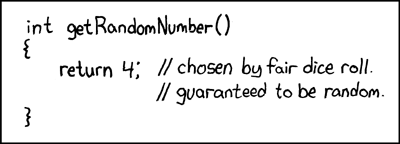
\includegraphics[width=\textwidth]{images/random_number}
}{Randall Munroe, \url{http://xkcd.com/221/}}
% random: http://xkcd.com/221/

This chapter covers the details of the derivation of some equations.



%% Section %%%%%%%%%%%%%%%%%%%%%%%%%%%%%%%%%%%%%%%%%%%%%%%%%
\section{Mathematical proofs}
\label{app:mathProofs}


% ----------------------------------------------------------------------
\subsection{Preliminary observations}

\begin{gather}
	\mathbf{B} : \nabla\overbar{\mathbf{u}} =  - 2 \nu_{SGS} \left[ \mathbf{S} : \mathbf{S}
		+ \mathbf{S} : \Tskew(\mathbf{\nabla\mycdot\mathbf{u}}) \right] 
		\label{eq:lesKEqProductionTermProofTmp03} \\
	\intertext{The contraction of a symmetric and a skew tensor vanishes by definition}
	\underbrace{\Tskew(\mathbf{T})}_{a_{ij}}:\underbrace{\Tsym(\mathbf{T})}_{s_{ij}} \\
	a_{ii} = 0 \\
	a_{ij} = -a_{ji} \\
	\Tskew(\mathbf{T}):\Tsym(\mathbf{T}) = a_{ij} s_{ij} = 0 \\
	\intertext{Thus, the second term in \eqref{eq:lesKEqProductionTermProofTmp03} vanishes.}
	\mathbf{B} : \nabla\overbar{\mathbf{u}} =  - 2 \nu_{SGS} \mathbf{S} : \mathbf{S} 
\end{gather}
